% % -----------------------------------------------------------------------------
\section{Overview of SBOL}
% % -----------------------------------------------------------------------------

Synthetic biology designs can be described using:
\begin{itemize}
\item Structural terms, e.g., a set of annotated sequences or information about the chemical makeup of components.
\item Functional terms, e.g., the way that components might interact with each other. 
\end{itemize}

As an example, consider an expression cassette, such as the one found in the plasmid pUC18~\cite{L08752.1}.
The system is designed to visually indicate whether a gene has been inserted into the plasmid: 
in the presence of IPTG, it expresses an enzyme that hydrolyses X-gal to form a blue product, but successful insertion disrupts the expression cassette and prevents the formation of this product. 
Internally, it has a number of parts, including a promoter, the lac repressor binding site, and the lacZ coding sequence.
These parts have specific component-level interactions with IPTG and X-gal, as well as native host gene products, transcriptional machinery, and translational machinery that collectively cause the desired system-level behavior.

In SBOL 3, both the structural and functional aspects are described using a class called \sbol{Component}, as depicted in \ref{images:overview1}.  
Namely, to represent structural aspects, a \sbol{Component} can include \sbol{Feature}s, some of which may be at some \sbol{Location} within a \sbol{Sequence}.  
A \sbol{Component} can also include \sbol{Constraint}s between these features.  
To represent functional aspects, a \sbol{Component} can include \sbol{Interaction}s that can refer to relationships between participating \sbol{Feature}s.  
Finally, a \sbol{Component} can have its behavior described using a \sbol{Model}.

\begin{figure}[ht]
\begin{center}
  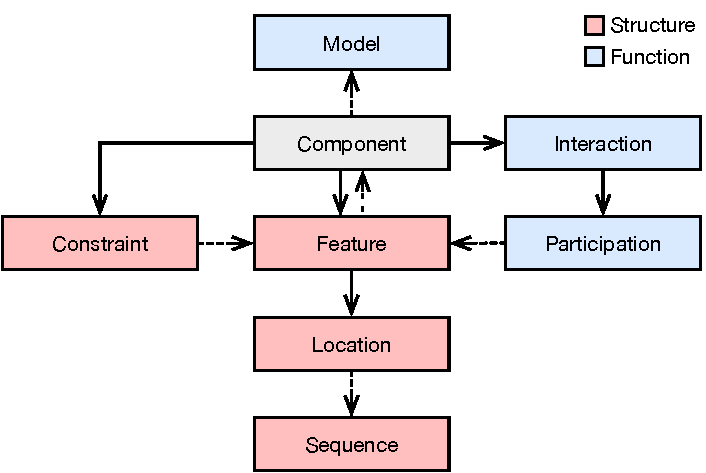
\includegraphics[scale=0.85]{images/SBOL3-main-classes.pdf}
\caption{The SBOL \sbol{Component} object and related objects.  
	Solid arrows indicates ownership, whereas a dashed arrow represents a reference to an object of another class.  
	Red boxes represent structural objects, while blue boxes represent functional objects.  
	To represent structural aspects, a \sbol{Component} can include \sbol{Feature}s, which may refer to \sbol{Location}s within a \sbol{Sequence}. 
	A \sbol{Component} can also include \sbol{Constraint}s between these features.  
	To represent functional aspects, a \sbol{Component} can include \sbol{Interaction}s that can refer to relationships between participating \sbol{Feature}s.  
	Finally, a \sbol{Component} can have its behavior described using a \sbol{Model}.}
\label{images:overview1}
\end{center}
\end{figure}

To continue with the pUC18 example, the description would begin with a top-level \sbol{Component} that represents the entire system.  
This \sbol{Component} specifies the structural elements that make up the cassette by referencing a number of \sbol{SubComponent} objects. These would include the DNA \sbol{SubComponent} for the promoter and the simple chemical
\sbol{SubComponent} for IPTG, for example.  
The \sbol{Component} objects can be organized hierarchically.  
For example, the plasmid \sbol{Component} might reference \sbol{SubComponent}s for the promoter, coding sequence, etc.  
Each \sbol{Component} object can also include the actual \sbol{Sequence} information (if available), as well as \sbol{SubComponent} objects that identify the \sbol{Location}s of the promoters, coding sequences, etc., on the \sbol{Sequence}.  
In order to specify functional information, the \sbol{Component} can also specify \sbol{Interaction} objects that describe any qualitative relationships among \sbol{SubComponent} \sbol{Participation}s, such as how IPTG and X-gal interact with the gene products.  Finally, a \sbol{Component} object can point to a \sbol{Model} object that provides a reference to a complete computational model expressed in a language such as SBML~\cite{SBML}, CellML~\cite{CellML}, or MATLAB~\cite{matlab}.

Whereas \ref{images:overview1} provides an overview of the classes used for describing designs within the SBOL 3 data model,  \ref{images:overview2} shows the rest of the classes used to describe the usage of a design within design-build-test-learn workflows in general.
In particular, designs can be expressed using \sbol{CombinatorialDerivation}s, \sbol{Component}s, and \sbol{Sequence}s.
These can describe not only genetic designs, but also designs for strains, multicellular systems, media, samples, etc.
A \sbol{CombinatorialDerivation} allows one to specify a design pattern where individual \sbol{SubComponent}s can be selected from a set of variants.  
The \sbol{Implementation} class is the build class, and it is used to represent physical artifacts like an actual sample of a plasmid.  
The \sbol{Experiment} and \sbol{ExperimentalData} classes are the test classes, allowing description of a collection of data generated in an experiment.  
The \sbol{Model} class, discussed earlier, associates learned information with a design.
The \prov{Activity} class is taken from the provenance ontology (PROV-O), which is described in~\ref{sec:provenance}.  For example, a build \prov{Activity} describes how an \sbol{Implementation} is constructed using a \sbol{Component} description.  On the other hand, a test \prov{Activity} describes how an \sbol{Experiment} is conducted using an \sbol{Implementation} artifact.  The \sbol{Collection} class has members, which can be of any of these types or \sbol{Collection}s themselves.  
Finally, all of these objects can refer to objects of the \sbol{Attachment} class, which are used to link out to external data (images, spreadsheets, textual documents, etc.). 
The next sections provide complete definitions and details for all of these classes.

\begin{figure}[ht]
\begin{center}
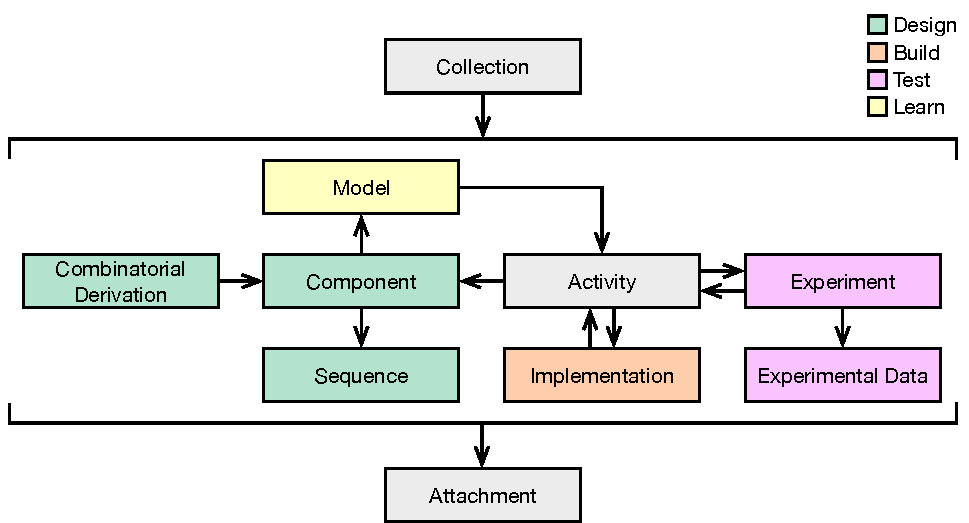
\includegraphics[scale=0.85]{images/SBOL3-top-levels.pdf}
\caption{Main classes of information represented by the SBOL 3 standard, and their relationships.  Green boxes represent design classes, orange boxes represent build classes, purple boxes represent test classes, yellow boxes represent learn classes, and the gray boxes represent additional utility classes.  Each of these classes will be described in more detail below.}
\label{images:overview2}
\end{center}
\end{figure}
